\documentclass[12pt, letterpaper]{report}
\usepackage{geometry}
\usepackage{times}
\usepackage{setspace}
\usepackage{titlesec}
\usepackage{graphicx}
\usepackage{float}
\usepackage{sectsty}
\usepackage[font=footnotesize]{caption}

\setlength\parindent{0pt}

\makeatletter
\renewcommand{\fnum@figure}{Fig. \thefigure}
\makeatother

\geometry{
letterpaper,
tmargin=23mm,
lmargin=23mm,
rmargin=23mm,
bmargin=23mm
}

\begin{document}
\thispagestyle{empty}

To: ENGR301\\
From: Team 2-4\\
\-\hspace{1.075cm} Anthony Bennett\\ 
Date: March 30, 2018\\
Subject: The Bit-Files - Proposal Edit

\paragraph*{\fontsize{14pt}{12pt}\selectfont Problem Statement \\  \fontsize{10pt}{12pt}\selectfont By: Anthony Bennett \\}
There is a low interest in Computer Science and Electrical Engineering in K-12 education while there is a growing need of these graduates in industry. As technology develops and continues to grow in its use, more jobs will be needed to maintain that growth. According to the Bureau of Labor Statistics (BLS), the expected job growth rate of Software Developers is 24\%, which indicates a growth much faster than average [BLS.gov, website]. As such, if these jobs are not filled, they will slow the development of technology. This is detrimental to the economy as more countries will be able to compete with the U.S. in terms of economic growth. 

\paragraph*{Global Comparison of U.S. to other countries \\ }
According to the Washington Post, when the U.S. is compared to other countries it shows that the U.S. lacks in major areas of educational development within our K-12 system regarding literacy, mathematics, and computer skills [Washington Post, website]. Figure 1 shows a chart regarding problem solving scores between developed first world countries that have access to technology-rich environments. 

\begin{figure}[H]
    \centering
    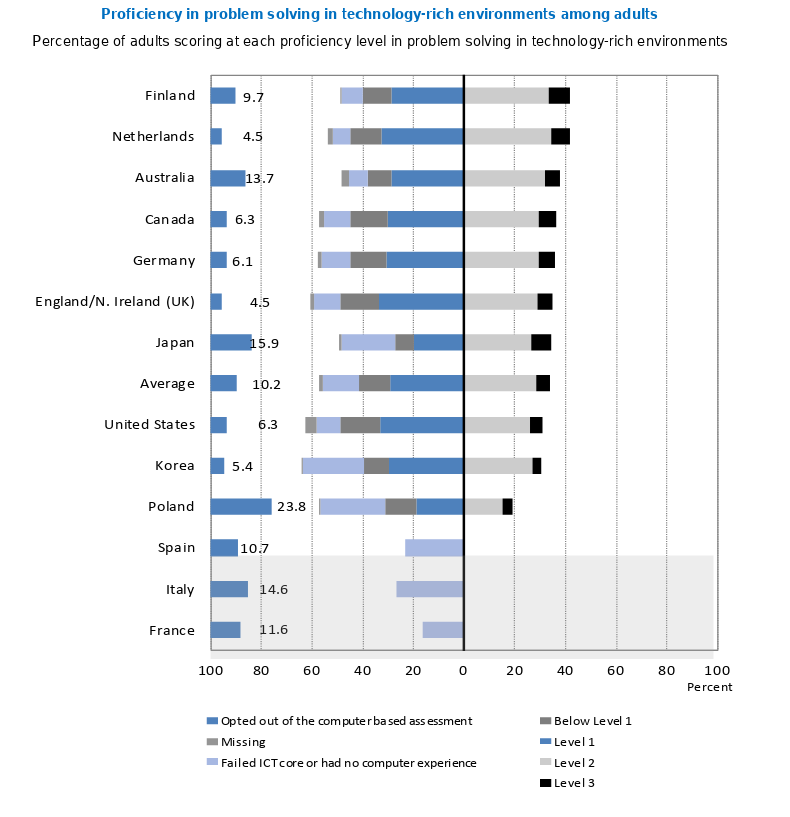
\includegraphics[scale=0.75]{figure1.png}
    \captionsetup{justification=centering}
    \caption{This chart represents proficiency in problem solving in technology-rich environments among adults with comparisons among countries around the globe [OECD, website]}
\end{figure}

Analysis of this chart shows that the U.S. lags behind most countries that were tested, scoring below the average. Other countries that had access to technology-rich environments had their adults score higher in problem solving skills. According to Code.org, Computer Science education has a significant impact on other skills than problem solving, such as mathematics and reading comphrension skills [Code.org, website]. Figure 2 shows this relationship between improved mathematics scores and Computer Science. Investing resources into Computer Science education would prove beneficial for society as it would help us boost our education rankings and the U.S. could show itself as a highly educated country to the world. \\

\begin{figure}[H]
    \centering
    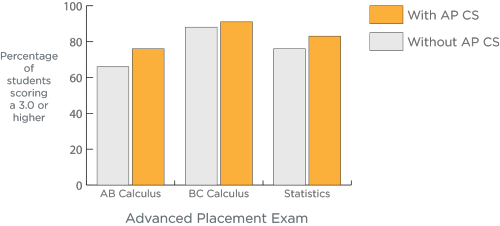
\includegraphics[scale=0.85]{figure13.png}
    \captionsetup{justification=centering}
    \caption{This chart demonstrates the relationship between taking AP Calculus exams with results from students who took AP Computer Science and who did not [Code.org, website]}
\end{figure}

\paragraph*{Missing in Curriculum\\}

Computer Science education has a beneficial impact on society by improving all skills regarding mathematics, reading, and literacy. However, Computer Science education is not offered as an option in many K-12 schools, having only 22\% offering it as an AP course that can be taken [Recode, website]. According to AP data from CollegeBoard, only 60,000 students have taken the AP Computer Science exam while over 300,000 have taken the Calculus AB exam [CollegeBoard, website]. More students would be willing to take AP Computer Science if it was offered. Expanding Computer Science education in K-12 high schools would be beneficial to society as it does lead to more students taking Computer Science to university if it is taken as a class in high school [Code.org, website]. 

\paragraph*{Soundness of references \\}
References used in this paper include the BLS.gov which is a website from the Bureau of Labor Statistics which compiles statistics for multiple jobs and job trends in the industry. This source is considered sound due the Bureau's main job to collect statistics and not to conclude on said statistics. The Washington Post and Recode are references used in this paper which their sources are considered unsound as they may have a bias as it is not stated on their site the negatives of increasing Computer Science education, only the negatives. Another resource used is Code.org which is an organization that sponsors Computer Science education and spreads awareness. Their source would be considered sound as their sources are from studies done by researchers at universities or think tanks which present unbiased data. The last two references used are CollegeBoard which is a non-profit which provides easier access to colleges and universities and OECD which is an international organization with 35 member countries that does studies on economic issues around the world. These sources are considered sound as well since their data is also unbiased with no opinion used as conclusive. 

\paragraph*{Improvement on Computer Science Education \\}
AP Data from CollegeBoard shows that more students are enrolling in AP Computer Science every year [CollegeBoard, website]. Figure 3 shows the increasing amount of AP Computer Science exams being taken every year, showing the booming popularity of the subject with high school students. AP Computer Science education is becoming cheaper to teach as organizations such as Code.org are partnering with companies such as Microsoft and Google to provide a free structured AP Computer Science course that is flexible to any school schedule. Having more resources available and having organizations such as Code.org spreading awareness on Computer Science education will heavily impact the growth of Computer Science graduates in a positive manner.

\begin{figure}[H]
    \centering
    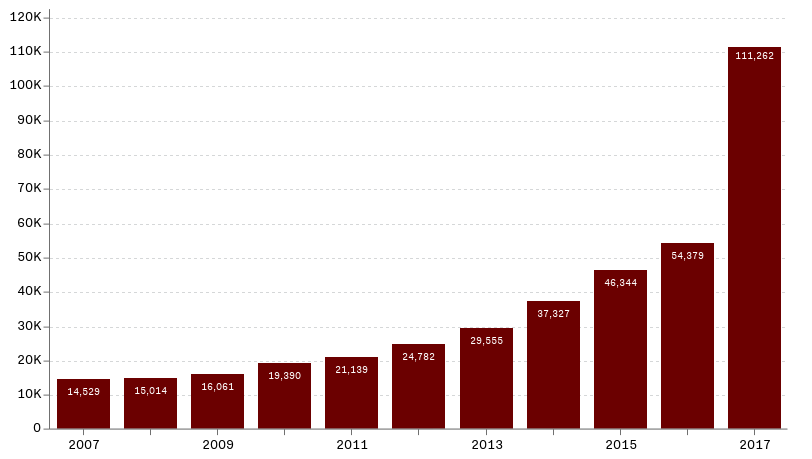
\includegraphics[scale=0.85]{figure14.png}
    \captionsetup{justification=centering}
    \caption{This chart shows the increasing number of students completing the AP Computer Science exams in high schools in the U.S. [Recode, website]}
\end{figure}
\end{document}